\documentclass[
	parskip=half,
	a4paper,
]{scrarticle}

\usepackage{xcolor}
\definecolor{seeblau}{HTML}{00A9E0}
\definecolor{seegrau}{HTML}{9AA0A7}

\definecolor{seeblau1}{HTML}{CCEEF9}
\definecolor{seeblau2}{HTML}{A6E1F4}
\definecolor{seeblau3}{HTML}{59C7EB}
\definecolor{seeblau4}{HTML}{00A9E0}
\definecolor{seeblau5}{HTML}{008ECE}


\usepackage{graphicx}
\usepackage{amsmath}
\usepackage{subcaption}
\usepackage{wrapfig}
\usepackage[english]{babel}
\usepackage{blindtext}
\usepackage{microtype}
\usepackage{siunitx}
\usepackage[utf8]{inputenc}
\usepackage{csquotes}
\usepackage{nicefrac}
\usepackage[T1]{fontenc}
\usepackage{amsfonts}
\usepackage{amssymb}
\usepackage{tikz}
\usepackage{parskip}

\usepackage{libertinus, libertinust1math}
\usepackage[sfdefault]{biolinum}
\usepackage{roboto}

\setkomafont{disposition}{\normalfont\sffamily}

% set margins
\usepackage{geometry}
\geometry{
	a4paper,
	left=2.5cm,
	right=2.5cm,
	top=2.5cm,
	bottom=2.5cm
}

% caption
\usepackage{caption}
\captionsetup{
	% font={sf},
	labelfont={sf, bf, color=seeblau},
	labelsep=quad,
	labelformat=simple,
}

% links
\usepackage{hyperref}
\hypersetup{
	colorlinks=true,
	linkcolor=seeblau,
	citecolor=seeblau,
	urlcolor=seeblau,
	% hidelinks=true
}

% bibliography
\usepackage[
	style=numeric-comp, % comp = compressed 4,5,6,7 -> 4-7
	sorting=none,		% Sort by appearance
	% autocite = superscript,
	% backref=true,
	hyperref=true,
	url=true,
	maxbibnames=100
]{biblatex}

\usepackage{float}
% \floatplacement{figure}{h}
% \floatplacement{table}{H}

% loosen float placement rules
\renewcommand{\topfraction}{0.8}
\renewcommand{\bottomfraction}{.8}
\renewcommand{\textfraction}{0.1}
\renewcommand{\floatpagefraction}{.9}
% make floats less likely to be placed on a separate page
\setcounter{totalnumber}{9}
\setcounter{topnumber}{9}
\setcounter{bottomnumber}{9}

% decrease space between floats and text
\setlength{\textfloatsep}{0.25cm}
\setlength{\floatsep}{0.25cm}

% decrease space after disposition
\RedeclareSectionCommands[
	afterskip=1px
]{section, subsection, subsubsection}

\usepackage{adjustbox}

\usepackage{datetime}
\newdateformat{dotdate}{
	\twodigit{\THEDAY}.\twodigit{\THEMONTH}.\THEYEAR
}
\newdateformat{monthyeardate}{%
  \monthname[\THEMONTH] \THEYEAR}


% header and footer
\usepackage[
  markcase=noupper
]{scrlayer-scrpage}% activates pagestyle scrheadings automatically
\clearpairofpagestyles
\setkomafont{pageheadfoot}{\normalfont\sffamily}
\setkomafont{pagenumber}{\normalfont\sffamily}
% \chead*{\color{seegrau} Draft \dotdate\today}
\ofoot*{\pagemark}
\ohead*{\rightmark}


\usepackage{ifthen}
\newcommand{\markieren}[4]{
	\ifthenelse{\equal{#1}{}}{}{\adjustbox{padding=3pt, bgcolor=seeblau1, margin=-1pt}{\strut{\sffamily\robotoMedium{#1}}}\\}
  \ifthenelse{\equal{#2}{}}{}{\adjustbox{padding=3pt, bgcolor=seeblau2, margin=-1pt}{\strut{\sffamily\robotoMedium{#2}}}\\}
	\ifthenelse{\equal{#3}{}}{}{\adjustbox{padding=3pt, bgcolor=seeblau3, margin=-1pt}{\strut{\sffamily\robotoMedium{#3}}}\\}
	\ifthenelse{\equal{#4}{}}{}{\adjustbox{padding=3pt, bgcolor=seeblau4, margin=-1pt}{\strut{\sffamily\robotoMedium{#4}}}}
}

\addbibresource{../literature.bib}
\begin{document}

\title{Procedures for Hot Electron Measurements}
\author{Leon Oleschko}
\date{\dotdate\today}

\begin{titlepage}
    \sffamily
    \vspace*{3cm}
    {
        \fontsize{32}{32}
        \markieren{}{Hot Electron}{Thermal Emission}{Spectroscopy}
    }
    \vspace{.25cm}\\
    {
        \Large
        Leon Oleschko\\
        Supervised by Peter Baum
        \vspace{.05cm}\\
        \dotdate\today\\
        % \vspace{.25cm}\\
        % \normalsize
        Universität Konstanz
    }
    \vfill
    {
        \normalfont\normalsize

    }
    \vfill
    \begin{flushright}
        Available at \url{www.github.com/leoole100/projekt-praktikum}.
    \end{flushright}
\end{titlepage}

% {
% 	\sffamily
% 	\hypersetup{hidelinks}
% 	\tableofcontents
% }

\clearpage
\section{Introduction}
Ultrafast laser-matter interactions on femtosecond timescales create non-equilibrium electronic states that are fundamentally important for understanding energy dissipation in condensed matter systems. When intense femtosecond laser pulses interact with materials, they can generate populations of hot electrons with temperatures significantly exceeding the lattice temperature \cite{lui_ultrafast_2010}. 
These transient hot electron populations have lifetimes on the order of hundreds of femtoseconds \cite{stange_hot_2015} and represent a critical intermediate state in ultrafast energy transfer processes. 
Hot carrier dynamics have attracted considerable interest for applications in next-generation photovoltaics, ultrafast terahertz photodetectors, and photocatalytic hydrogen production \cite{tang_plasmonic_2020,konig_hot_2010}.

% Two temperature model
The process of heating a bulk material by means of femtosecond laser pulses can be described with a two-temperature model \cite{roob_thermal_2025}. In this framework, an external energy input first excites out-of-equilibrium electrons in the electron gas to a temperature $T_e$, while the lattice remains at an initial temperature $T_l$. For the short timescales relevant to hot electron dynamics, the lattice temperature can be assumed constant at room temperature, as thermal diffusion in the lattice occurs on much longer timescales than electron thermalization. Under this approximation, the temporal evolution of the electron temperature is governed by:
\begin{equation}
C_e(T_e) \frac{\partial T_e}{\partial t} = -G(T_e - T_l) + S(r,t)\text{,}
\end{equation}
where $C_e(T_e)$ is the temperature-dependent electronic heat capacity, $G$ is the electron-phonon coupling constant, $T_l$ is the constant lattice temperature, and $S(r,t)$ represents the laser source term. Since the electronic heat capacity $C_e$ is much lower than the lattice heat capacity, the hot electron temperature can far exceed the lattice temperature during the initial femtoseconds following laser excitation \cite{nihira_temperature_2003}. The cooling dynamics involve complex mechanisms including strongly coupled optical phonons \cite{kampfrath_strongly_2005} and phonon-mediated relaxation processes \cite{stange_hot_2015}.\\
Integration of this equation using realistic laser parameters predicts dramatic electronic temperature rises in graphite. \autoref{fig:temperature} shows the calculated time-dependent electron temperature for a \SI{7.5}{\micro J} pulse (\SI{300}{mW} average power at \SI{40}{kHz} repetition rate) with \SI{250}{fs} FWHM duration focused to a \SI{50}{\micro m} diameter spot \cite{roob_thermal_2025}. The simulation demonstrates peak electronic temperatures exceeding \SI{6000}{K}, far above the lattice temperature, with cooling occurring on sub-picosecond timescales through electron-phonon coupling.
\begin{figure}[hb]
    \centering
    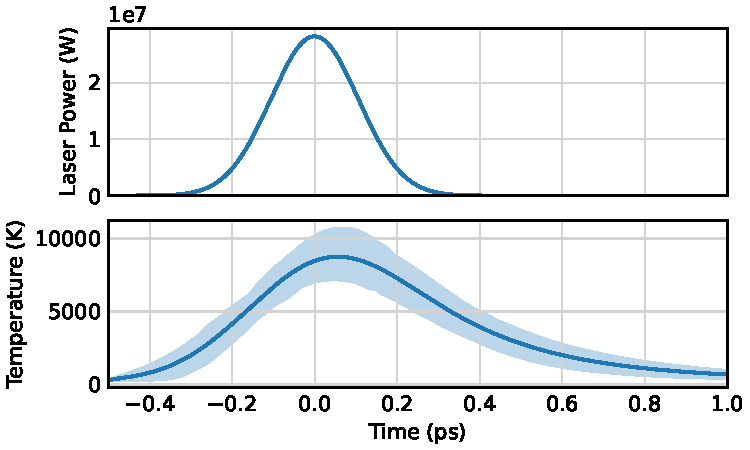
\includegraphics{../analysis/figures/model te.pdf}
    \caption{Calculated electron temperature evolution following femtosecond laser excitation of graphite, showing rapid heating and subsequent cooling through electron-phonon coupling.}
    \label{fig:temperature}
\end{figure}

% thermal radiation
The hot electrons described by the two-temperature model emit thermal radiation during their cooling process. The spectral energy density of this radiation follows Planck's law:
\begin{equation}
B(\lambda, T) = \frac{2hc^2}{\lambda^5} \frac{1}{\exp\left(\frac{hc}{\lambda kT}\right) - 1}
\end{equation}
where $h$ is Planck's constant, $c$ is the speed of light, $k$ is the Boltzmann constant, and $T$ is the electron temperature. Since hot electron temperatures reach values of several thousand Kelvin and far exceed lattice temperatures during femtosecond excitation, the thermal radiation spectrum of hot electrons dominates over that of the lattice. 

For the time-dependent electron temperature $T_e(t)$ predicted by the two-temperature model, the total thermal radiation spectrum is obtained by integrating Planck's law over the entire cooling dynamics. \autoref{fig:model_spectrum} shows the calculated spectrum for the same laser parameters as before. The predicted spectrum exhibits a broad emission band spanning visible and near-infrared regions, with peak emission around \SI{500}{nm} corresponding to the high electron temperatures achieved.
\begin{figure}[b]
    \centering
    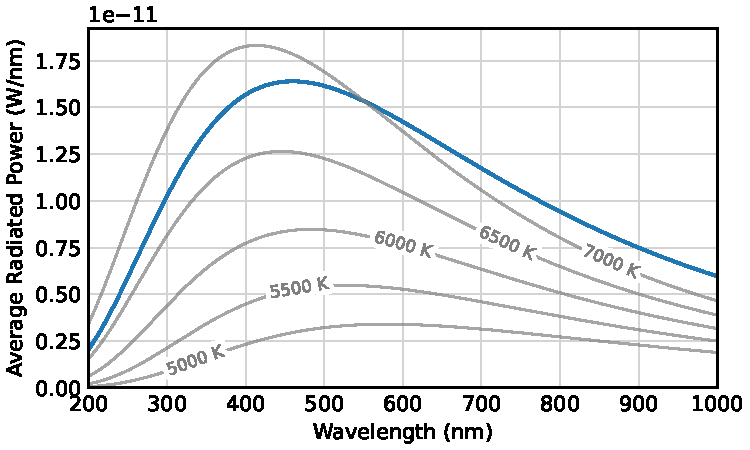
\includegraphics{../analysis/figures/model spectrum.pdf}
    \caption{Calculated thermal radiation spectrum from hot electrons in graphite, obtained by integrating Planck's law over the time-dependent electron temperature cooling dynamics. The broad spectrum peaks in the visible range due to the high electron temperatures achieved.}
    \label{fig:model_spectrum}
\end{figure}

% experimental context
The theoretical predictions from the two-temperature model indicate that thermal radiation from hot electrons should produce a low power, broadband spectrum spanning the visible and near-infrared regions. Building upon this understanding, Roob conceptualized a experimental setup to measure the thermal radiation of the hot electrons \cite{roob_thermal_2025}. The ultrafast hot electrons are characterized by their emitted thermal radiation, utilizing graphite as the sample material due to its well-characterized electronic properties \cite{nihira_temperature_2003} and easy procurement.

% my specific work
The present internship work focuses on the optimization and calibration of the experimental setup developed by Roob \cite{roob_thermal_2025}. The primary objective was to improve the measurement of thermal emissions from ultrafast hot electrons through systematic characterization of noise sources in EMCCD detection systems \cite{andor_establishing_nodate, dr_jo_walters_sensitivity_2023} and calibration of the quantum efficiency of the spectrometer system. 
This report presents the experimental setup optimization, noise analysis, and theoretical framework for spectrometer calibration.

\clearpage
\section{Experimental Setup}

\begin{figure}[hb]
    \centering
     \begin{subfigure}{4in}
        \centering
        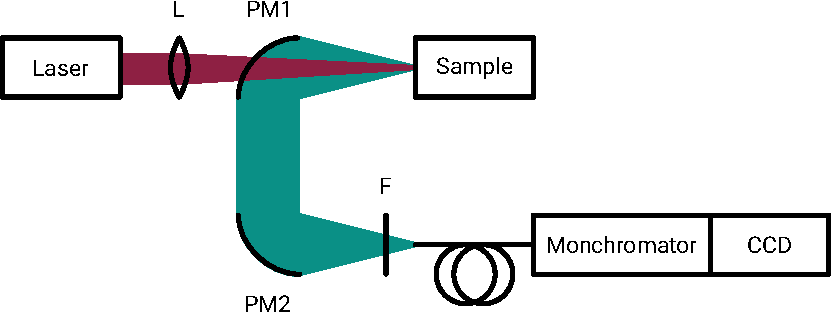
\includegraphics{figures/setup.pdf}
        \caption{Schematic}
    \end{subfigure}
    \hfill
    \begin{subfigure}{2in}
        \centering
        \includegraphics{figures/photo_setup.pdf}
        \caption{Image}
    \end{subfigure}
    \label{fig:setup}
    \caption{Experimental Setup.}
\end{figure}

The experimental setup, designed by Leon Roob \cite{roob_thermal_2025}, is shown schematically in \autoref{fig:setup}. This broadband photoemission configuration enables measurement of thermal emission from ultrafast hot electrons.

The excitation source is a Pharos PH1-20 laser (Light Conversion) operating at \SI{1030}{nm} wavelength with \SI{250}{fs} FWHM pulse duration and \SI{100}{kHz} repetition rate. The beam undergoes 4-axis stabilization and is expanded to a diameter of \SI{5}{mm} upon entering the experimental chamber. A focusing lens (L) with \SI{200}{mm} focal length creates a diffraction-limited spot size of $4\lambda f / \pi D = \SI{50}{\micro m}$ on the sample surface.

Upon laser excitation, the sample absorbs the pulse energy and emits thermal radiation into the collection hemisphere. The broadband emission is collected using UV-enhanced aluminum-coated off-axis parabolic mirrors (PM). Mirror PM1 (\SI{50}{mm} focal length) collects the emission, while PM2 (\SI{101}{mm} focal length) focuses the light through a spectral filter onto a bare multimode fiber end.
This mirror configuration provides a magnification of $f_\text{PM2}/f_\text{PM1} = 2$ for the collected thermal emission. Therefore the spotsize is roughtly \SI{100}{\micro m} in diameter.

The optical fiber (QP200-2-SR-BX, Ocean Optics) is a \SI{200}{\micro m} core multimode fiber optimized for 300--1100\,nm transmission. Spectral analysis employs an Acton SpectraPro 300i monochromator equipped with a 150\,lines/mm grating blazed at \SI{500}{nm}. Detection utilizes an Andor iXon$^\text{EM}$+ 897 EMCCD camera operated in vertical binning mode as a line detector.

For alignment optimization, lens L, the sample, and fiber end are mounted on 3-axis translation stages, while the parabolic mirrors remain fixed.

\section{Characterization of Noise Sources}

Detecting the weak thermal radiation from hot electrons requires careful optimization of the signal-to-noise ratio (SNR). The dominant noise sources originate from the detector, while laser power fluctuations are assumed negligible.

The EMCCD detector exhibits several characteristic noise mechanisms well-documented by Andor \cite{andor_establishing_nodate,dr_jo_walters_sensitivity_2023} and detailed in \cite{european_machine_vision_association_standard_2010}.

\textbf{Readout noise} represents the fundamental noise floor, arising from charge transfer operations and analog-to-digital conversion. For this high-performance CCD, readout noise measures approximately \SI{1}{e^-} \cite{andor_ixonem_nodate}, consistent with measurements shown in \autoref{fig:dark_noise}. Since this noise applies per readout bin rather than per pixel, hardware vertical binning effectively reduces its impact.

\begin{figure}[hb]
    \centering
    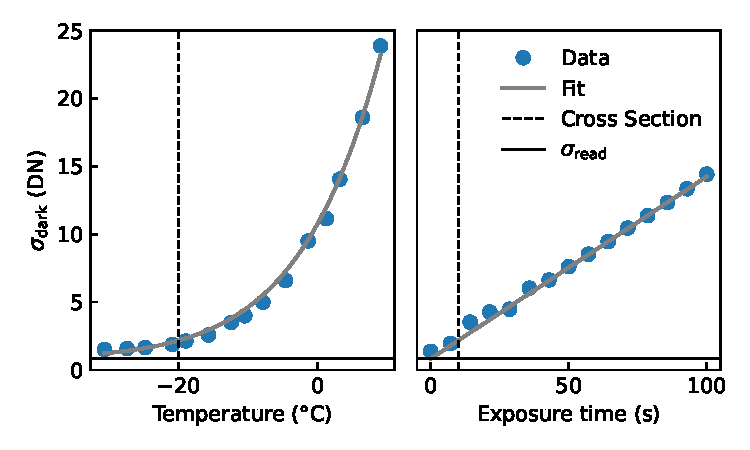
\includegraphics{../analysis/figures/dark_noise.pdf}
    \caption{Dark noise as a function of sensor temperature and exposure time. The fitted curve yields an effective activation energy of $E = \SI{0.597(4)}{eV}$ and constant readout noise of $\sigma_{\text{read}} = \SI{0.81(12)}{e^-}$.}
    \label{fig:dark_noise}
\end{figure}

\textbf{Dark current noise} results from thermal excitation of electrons within the detector semiconductor, following the relationship $N_\text{dark} \propto \exp(-E / kT) \cdot t_\text{exp}$, as demonstrated in \autoref{fig:dark_noise}. Cooling the detector to \SI{-80}{\degreeCelsius} effectively suppresses this contribution, rendering it negligible for typical exposure times.

\textbf{Clock-induced charge noise} scales with electron multiplication gain and signal amplitude. Therefore, sensor gain is deactivated when signal levels significantly exceed readout noise \cite{andor_establishing_nodate}, as in the present configuration.

\begin{figure}
    \centering
    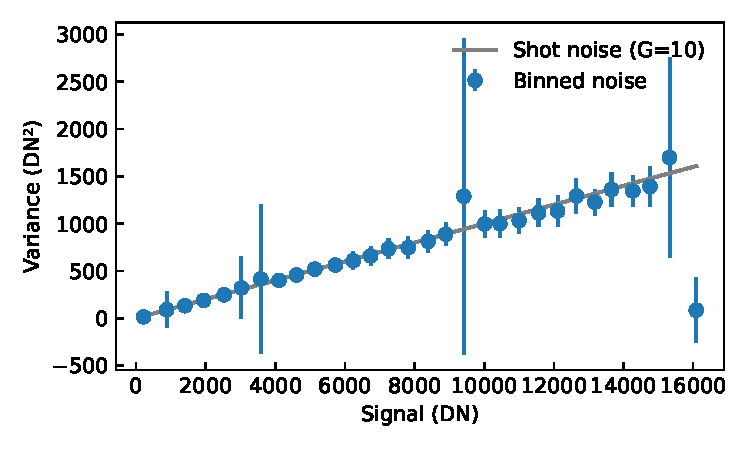
\includegraphics{../analysis/figures/shot noise.pdf}
    \caption{Measured noise versus signal, demonstrating shot noise-limited performance.}
    \label{fig:shotnoise}
\end{figure}

Under these optimized conditions, \textbf{shot noise} becomes the dominant limitation, establishing shot noise-limited operation as shown in \autoref{fig:shotnoise}. \textbf{TODO}

\section{Efficiency and Flatness}

The detection efficiency—defined as the fraction of sample-emitted light reaching the detector—varies with wavelength due to component-specific spectral responses.

The parabolic mirrors and optical fiber exhibit relatively flat spectral responses across the detection range, contributing primarily constant efficiency factors. However, other components introduce wavelength-dependent losses that must be characterized.

\begin{figure}[hb]
    \centering
    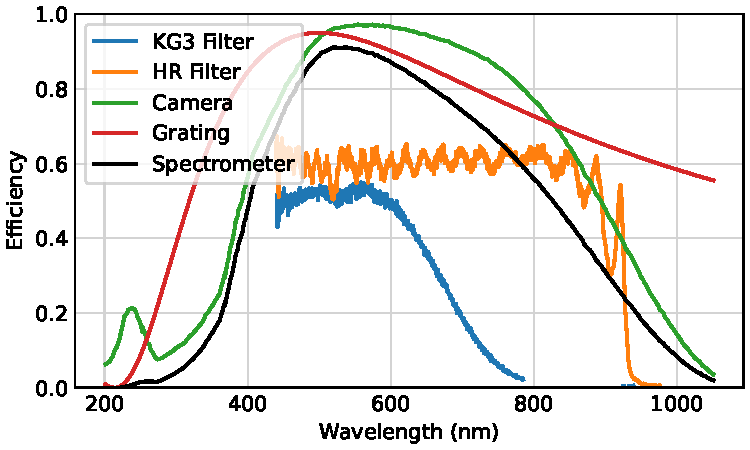
\includegraphics{../analysis/figures/filter.pdf}
    \caption{Spectral efficiency of various optical components and filters employed in the setup.}
    \label{fig:efficiency}
\end{figure}

Spectral filters for laser rejection exhibit distinct transmission characteristics, as shown in \autoref{fig:efficiency}. The SCHOTT KG3 filter, designed for infrared absorption, displays a gradual transmission edge that attenuates expected thermal emission. The HR filter, identified as a dielectric shortpass filter (likely Edmund Optics), shows sharper cutoff behavior, though detailed specifications were unavailable.

The detector quantum efficiency and grating efficiency curves require more sophisticated characterization. \autoref{fig:efficiency} presents the manufacturer-specified quantum efficiency for the EMCCD camera. Grating efficiency calculations employ the blazed grating model from \cite{barker_ripple_1984}, accounting for wavelength-dependent diffraction characteristics.

\subsection{Calibration}
Spectrometer efficiency calibration requires a reference source with precisely known spectral characteristics. This process is distinct from wavelength calibration, which establishes the correct mapping between detector pixels and wavelengths. Wavelength calibration procedures are well-documented and readily available in monochromator manuals and are therefore omitted from this discussion. The standard approach for efficiency calibration employs calibrated tungsten-halogen lamps with traceable spectral irradiance standards.

Professional calibration laboratories employ monochromator-based spectral comparator facilities that use silicon photodiode trap detectors previously calibrated against NIST's cryogenic electrical substitution radiometers \cite{houston_achievement_2022,larason_nist_1996}. This approach enables spectral responsivity calibrations with uncertainties below 0.1\% across the visible and near-infrared spectrum.

\begin{figure}[hb]
    \centering
    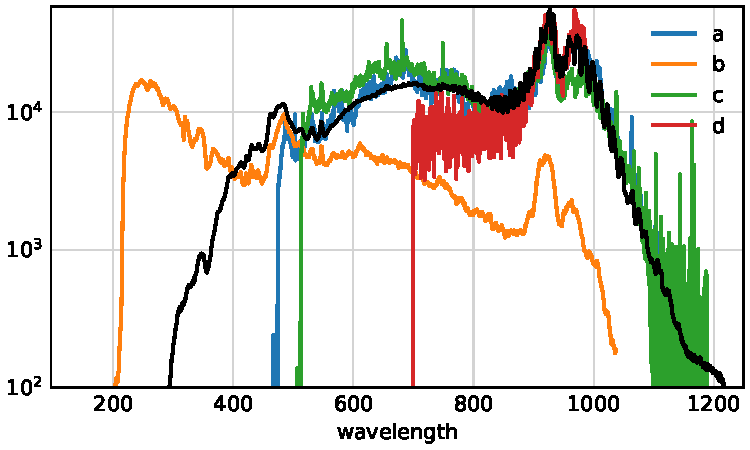
\includegraphics{../analysis/figures/efficiency_different.pdf}
    \caption{Comparison of identical spectra recorded with different uncalibrated spectrometer systems, demonstrating the calibration discrepancies that arise without proper reference standards.}
    \label{fig:calibration}
\end{figure}

Since no calibrated light source or reference detector with known spectral response was available for this work, an alternative approach using multiple uncalibrated Ocean Optics USB spectrometers was attempted. The broad-spectrum output of a deuterium-halogen lamp (DH-2000-BAL, Ocean Optics) was measured with several different spectrometers to assess consistency. \autoref{fig:calibration} shows the resulting spectra with intensity scaling adjusted for the different instrument sensitivities. The significant disagreement between instruments demonstrates the inadequacy of this approach and underscores the necessity for calibration against traceable reference standards. This comparison illustrates why professional-grade calibration requires the rigorous procedures and metrologically traceable standards maintained by national institutes, rather than relative comparisons between uncalibrated instruments.

\clearpage
\section{Data Analysis and Spectral Modeling}
\begin{figure}
    \centering
    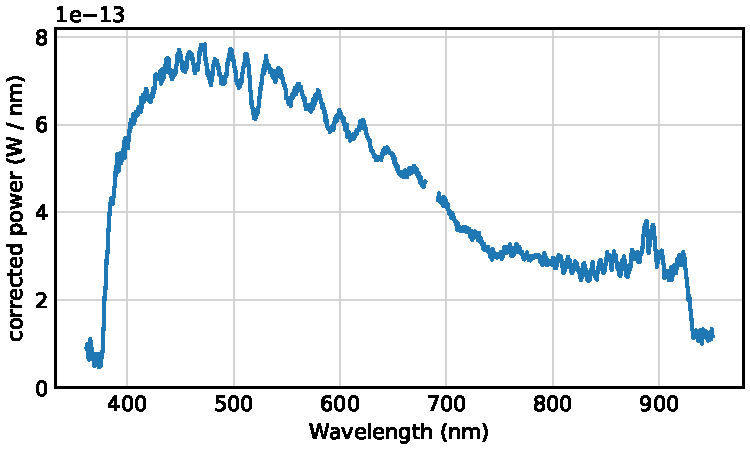
\includegraphics{../analysis/figures/corrected spectrum.pdf}
    \caption{}
\end{figure}

\clearpage
\section{Conclusion}

\clearpage
\printbibliography

\end{document}